
% This LaTeX was auto-generated from MATLAB code.
% To make changes, update the MATLAB code and republish this document.

\documentclass{article}
\usepackage{graphicx}
\usepackage{color}

\sloppy
\definecolor{lightgray}{gray}{0.5}
\setlength{\parindent}{0pt}

\begin{document}

    
    \begin{verbatim}
close all
clear all
%Lab 1 - ICT HEALTH - Perform regression - MSE

load('data_train_norm.mat');
load('data_test_norm.mat');

F0 = 7;
flag_features = 4; %first features

y_train = data_train_norm(:,F0);
y_test = data_test_norm(:,F0);

X_train = data_train_norm(:,flag_features:end);
X_test = data_test_norm(:,flag_features:end);
X_train(:,F0-flag_features) = [];
X_test(:,F0-flag_features)=[];

% Estimate a_hat
a_hat = inv(transpose(X_train)*X_train)*transpose(X_train)*y_train;
y_hat_train = X_train * a_hat;
y_hat_test = X_test * a_hat;

figure
plot(y_hat_train)
hold on
plot(y_train, '--k')
axis([0 840 -2 18])
grid on
legend('y\_hat\_train', 'y\_train', 'Location', 'northwest')
title('y\_hat\_train vs y\_train')

figure
plot(y_test)
hold on
plot(y_hat_test, '--k')
axis([0 150 -1.75 3.5])
grid on
legend('y\_hat\_test', 'y\_test')
title('y\_hat\_test vs y\_test')

[N,X] = hist(y_hat_train - y_train, 50);
figure
hist(y_hat_train - y_train, 50)
grid on

[N2,X2] = hist(y_hat_test - y_test, 50);
figure
hist(y_hat_test - y_test, 50)
grid on
\end{verbatim}

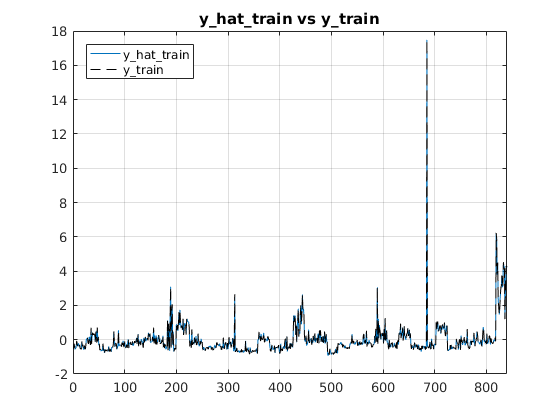
\includegraphics [width=4in]{Lab1Part3_01.png}

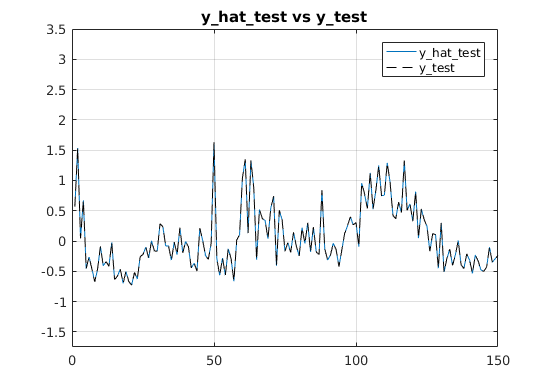
\includegraphics [width=4in]{Lab1Part3_02.png}

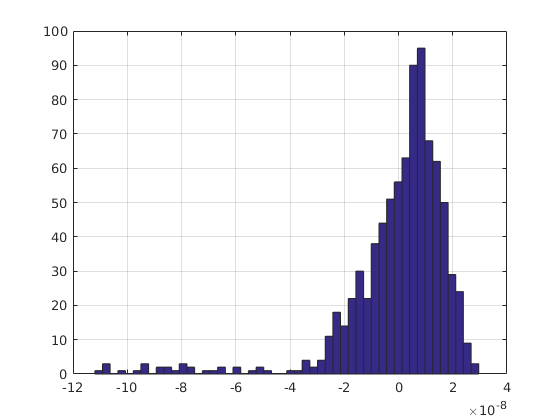
\includegraphics [width=4in]{Lab1Part3_03.png}

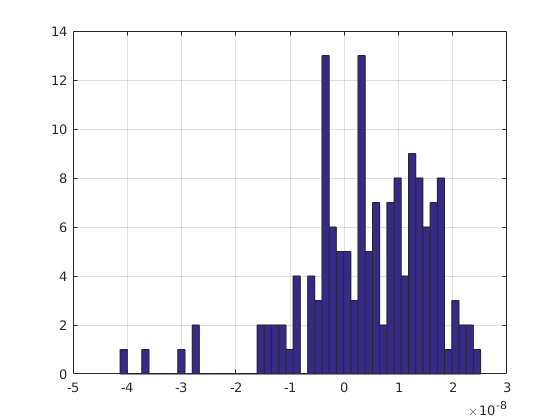
\includegraphics [width=4in]{Lab1Part3_04.png}



\end{document}
    
